\providecommand{\main}{../../../..}
\documentclass[\main/dresen_thesis.tex]{subfiles}
\begin{document}
  \label{sec:monolayers:nanoparticle:sans}

    By using small-angle neutron scattering, the oleic acid shell thickness can be determined, and by using polarized neutrons the magnetization density of the nanoparticles is probed.

    \paragraphNewLine{SANS Model: Oleic Acid Shell and Micelles}
      % \reffig{fig:monolayers:nanoparticle:sans:initialSim} shows the data the simulation of the superball formfactor with the parameters obtained from SAXS, the SLD calculated for the same composition determined by XRD and EDX, and the assumption of a $1.5 \unit{nm}$ oleic acid shell, which is a size observed in literature for oleic acid ligated nanoparticles \cite{Disch_2012_Quant}.
      % The form factor is scaled to agree with the data initially to compare the trend of experimental and simulated data.

      % The comparison to the initial form factor model of the superball shows the maxima at the same scattering vector values, which tells that the nanoparticle size of the superball obtained from SAXS agrees with the size of the particle in SANS as expected.
      % The superball form factor, however, decreases faster in intensity than the actual data and can not be corrected by assuming only a constant background from incoherent scattering for example.
      % This hints to an additional background contribution that is dependent on the scattering vector.
      % Earlier SANS studies on oleic acid ligated nanoparticles \cite{Disch_2010_Thesp} observe something similar and explain this by assuming the formation of oleic acid micelles in dispersion, which would be nearly invisible for X-rays due to the small contrast of organic solvents with oleic acid, but have an observable effect in neutron scattering.

      % \begin{figure}[tb]
      %   \centering
      %   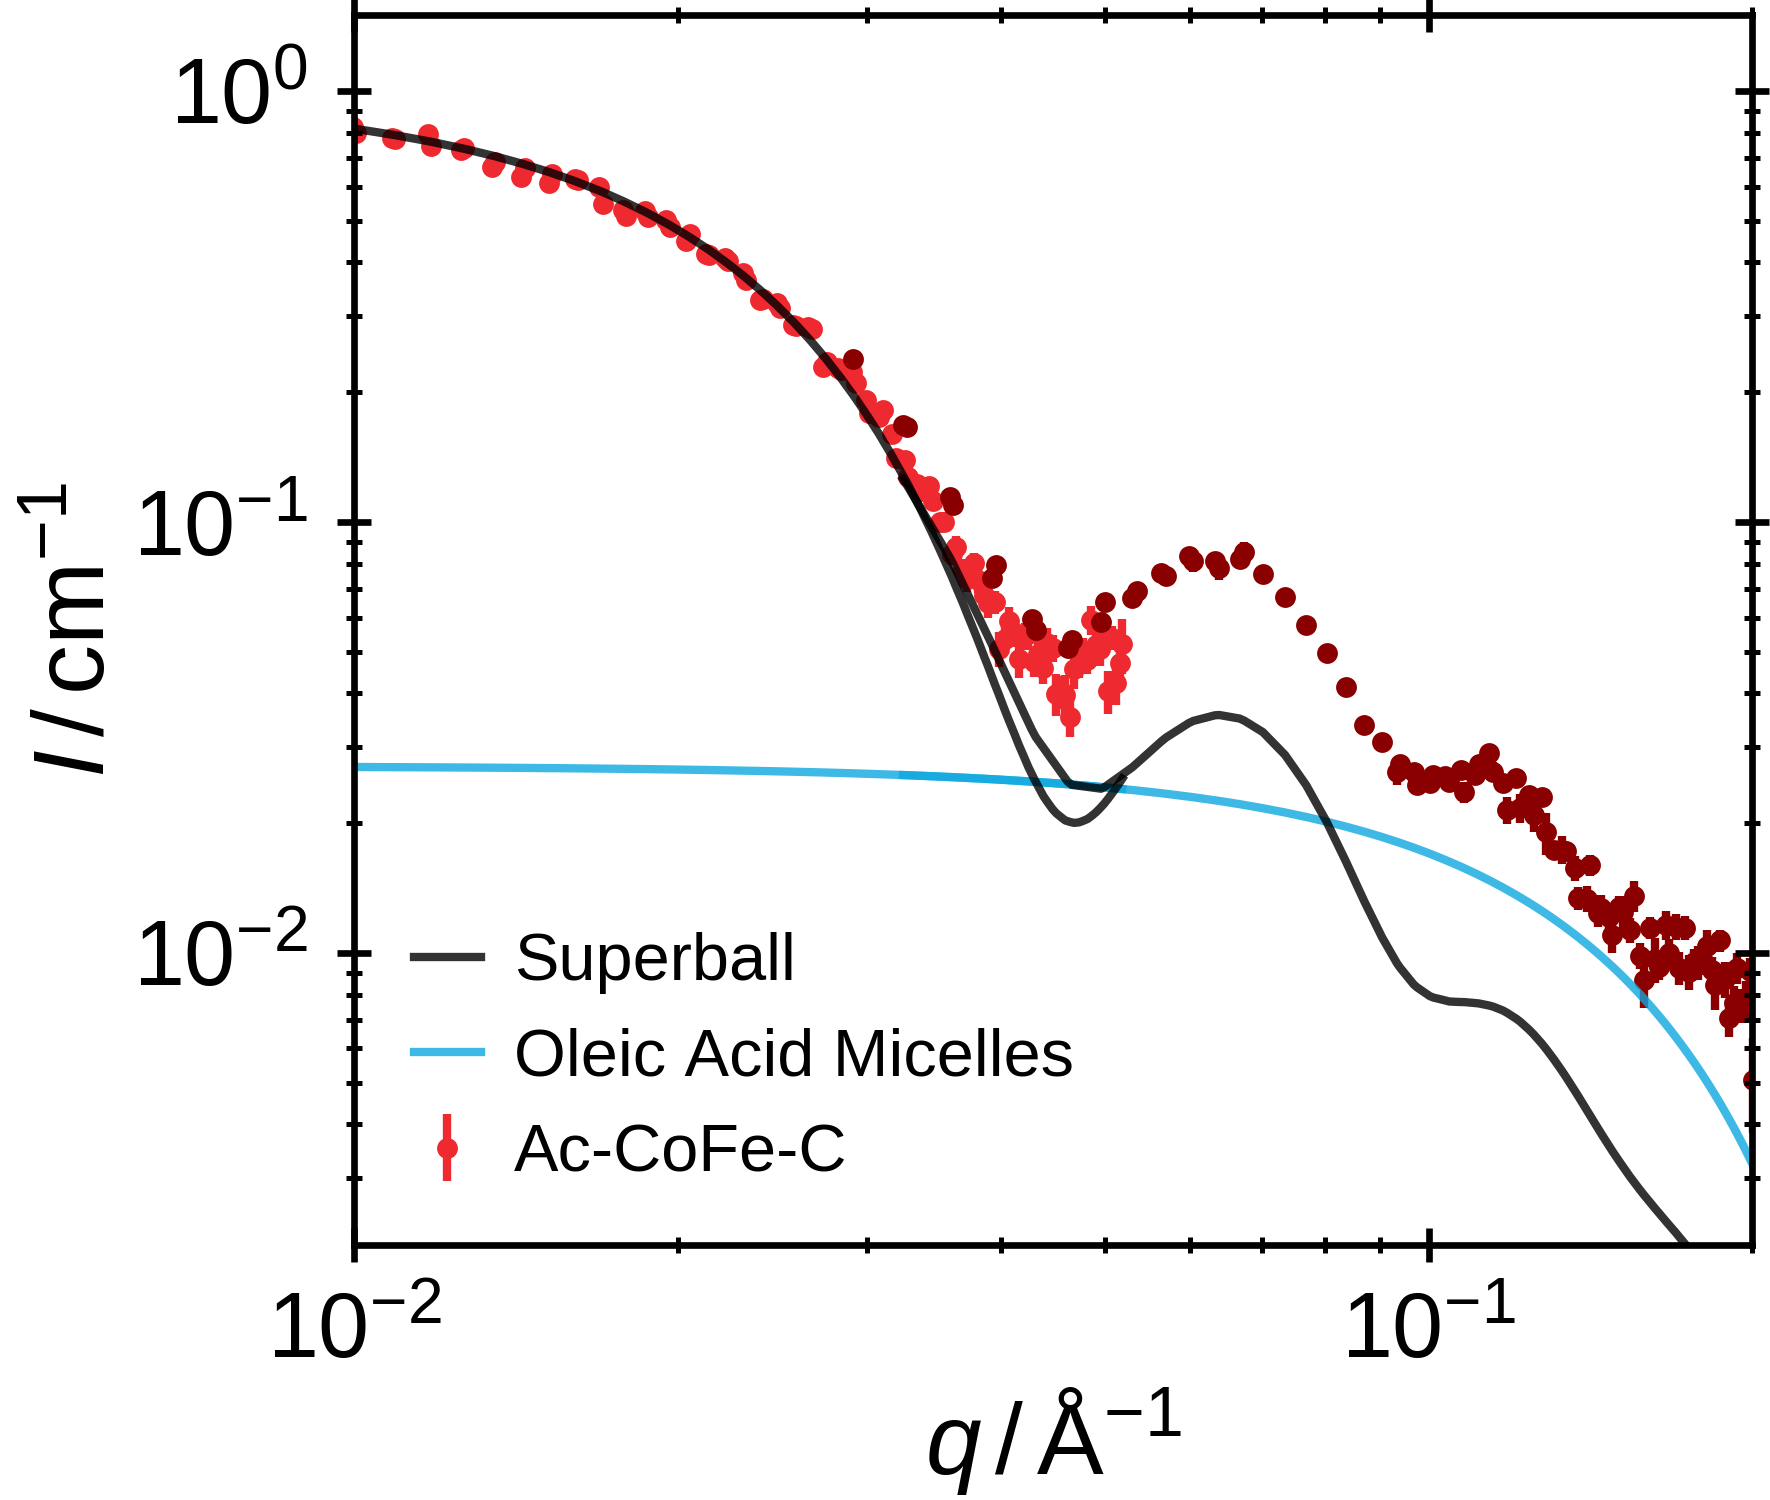
\includegraphics{monolayers_SAS_Ac_CoFe_C_InitialSANS}
      %   \caption{\label{fig:monolayers:nanoparticle:sans:initialSim}Initial superball form factor (black) before a fit to the SANS data of Ac-CoFe-C is performed using the parameters of the SAXS fit and by estimating the surfactant shell thickness from literature. The form factor, which would be produced by oleic acid micelles with a radius analogue to the shell thickness is shown in blue.}
      % \end{figure}

      The SANS data of Ac-CoFe-C in \reffig{fig:monolayers:nanoparticle:sans:superballOAFit} shows two visible form factor maxima and three minima positions can be estimated in it.
      The SANS data can be described by a sum of form factors, one from a superball with an oleic acid shell, and the other a spherical formfactor to model oleic acid micelles in the dispersion.
      As the nanoparticle size and shape is determined very well by SAXS, it is fixed in the superball form factor to the previously determined values and only the thickness $d$ of the superball's oleic acid shell is varied.
      The particle number density $n_\mathrm{NP}$ of the dispersion is also varied, as the particles were dried and redispersed for the measurement and therefore the concentration might have changed.
      The best fit is shown in \reffig{fig:monolayers:nanoparticle:sans:superballOAFit} and the varied parameters are tabulated in \reftab{tab:monolayers:nanoparticle:sans:superballOAFit}.
      The inset of \reffig{fig:monolayers:nanoparticle:sans:superballOAFit} shows the scattering length density profiles to visualize the length scales of the core and shell size.
      For the superball the shown SLD profile represents a cut along one of the four fold axis.

      \begin{figure}[tb]
        \centering
        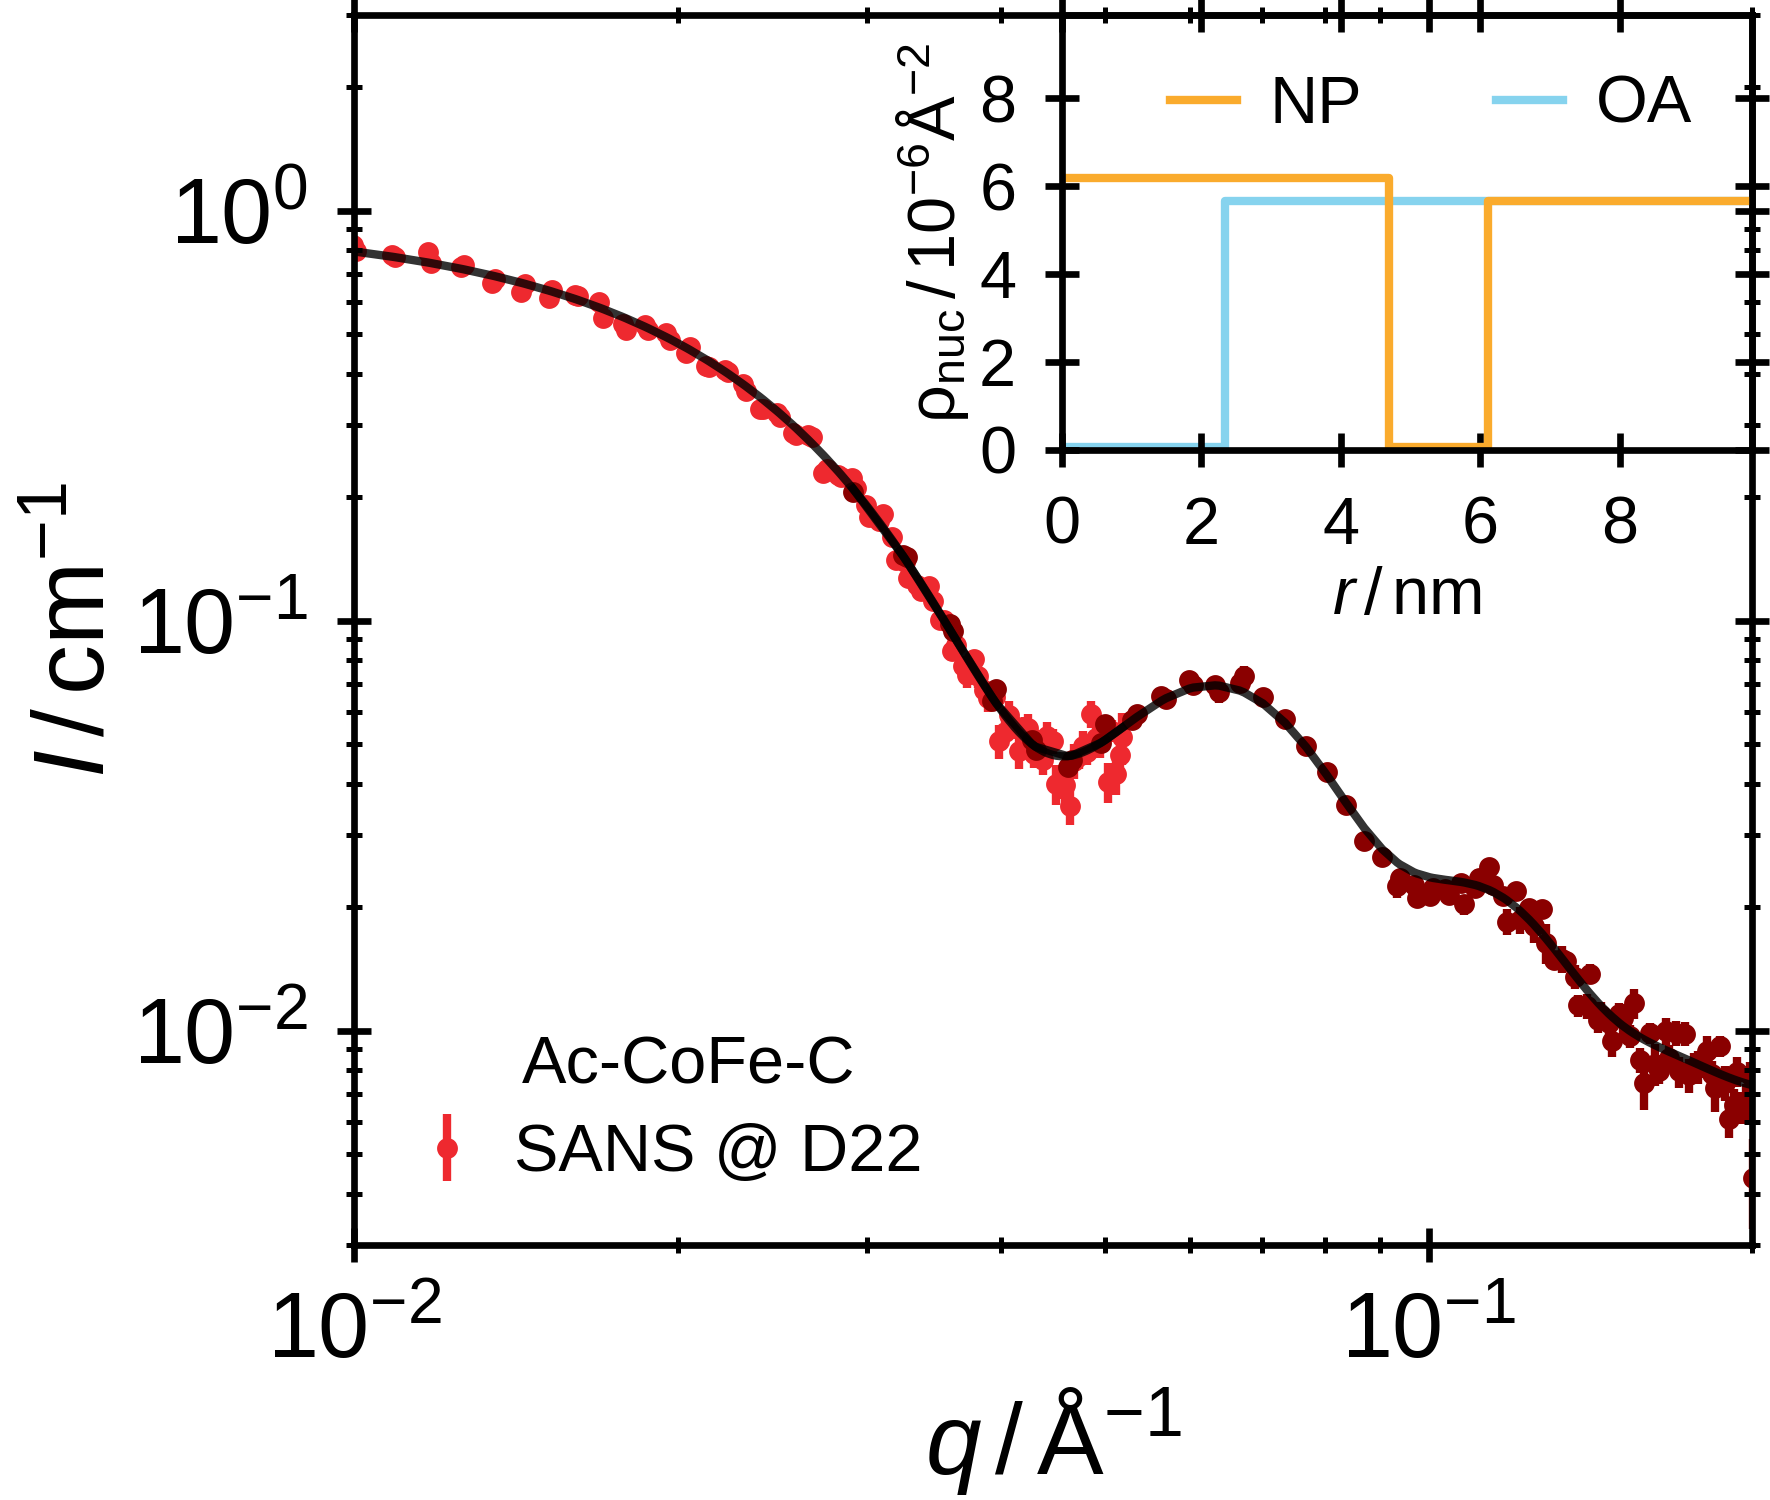
\includegraphics{monolayers_SAS_Ac_CoFe_C_SANS}
        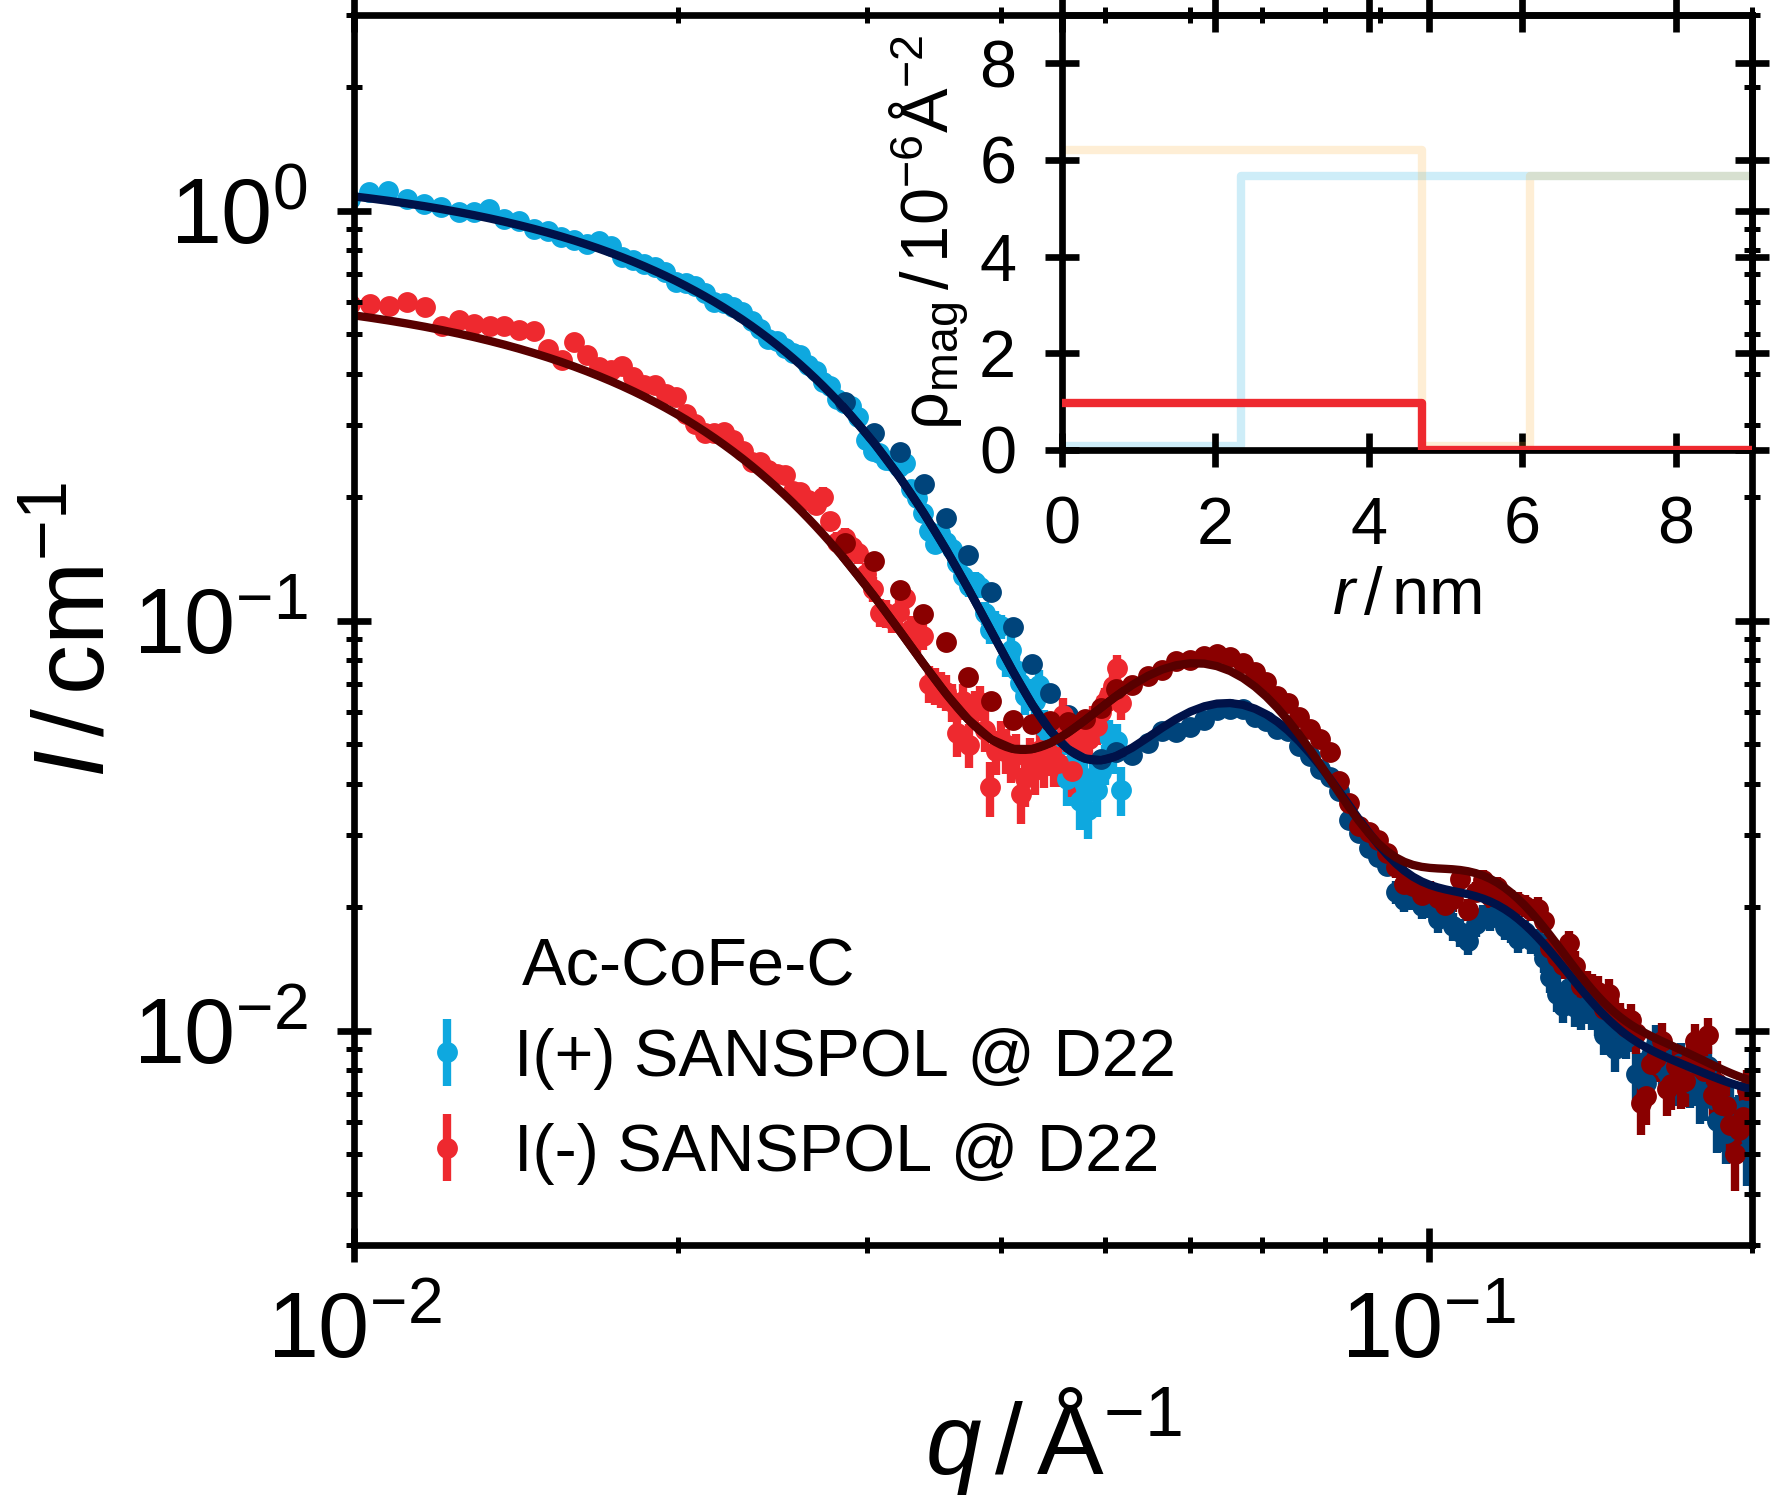
\includegraphics{monolayers_SAS_Ac_CoFe_C_SANSPOLFit}
        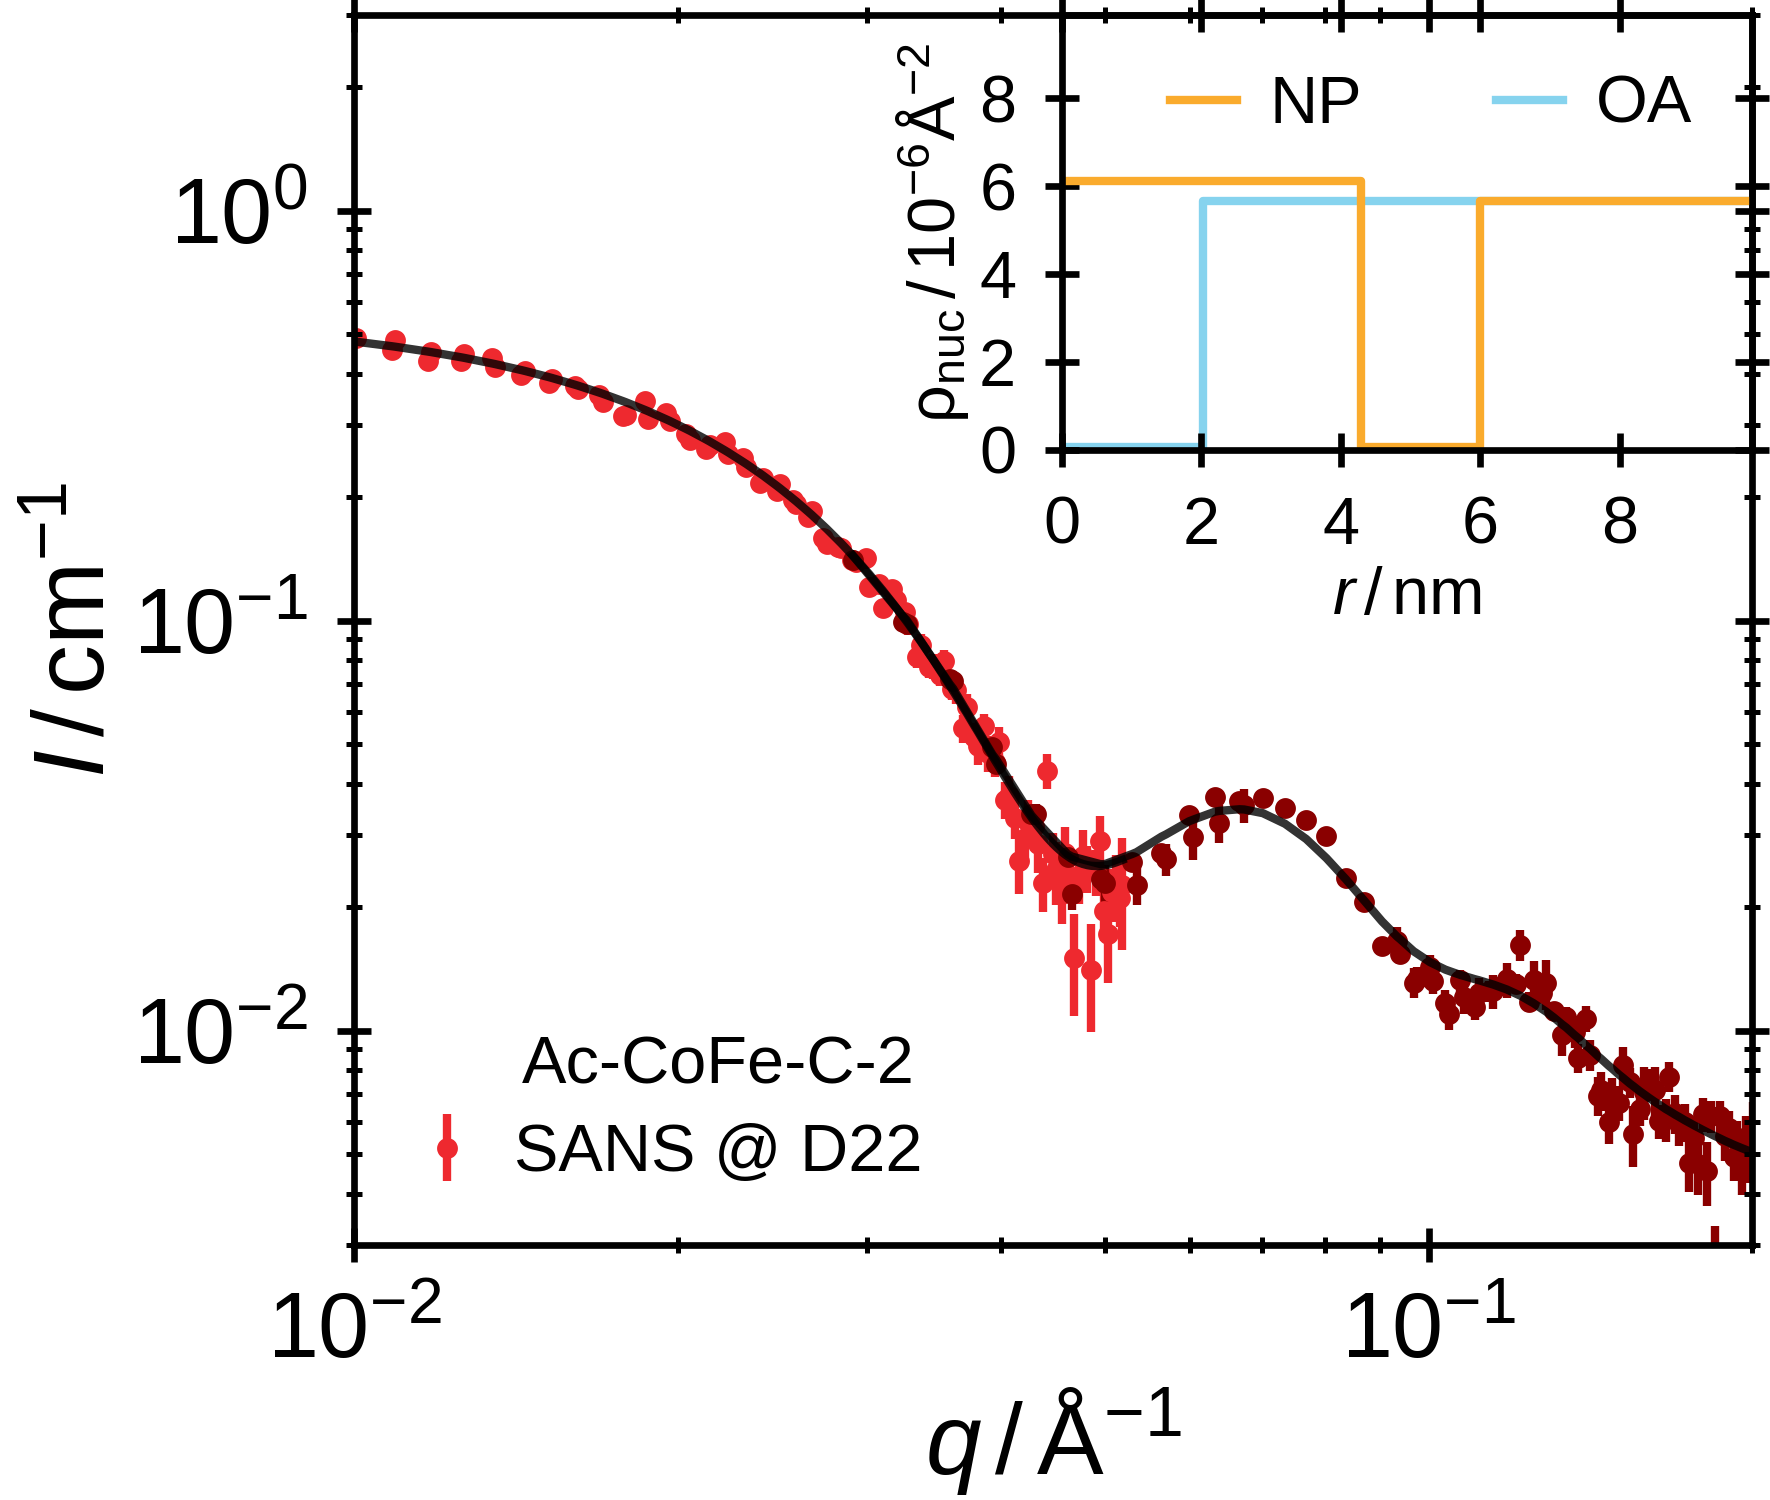
\includegraphics{monolayers_SAS_Ac_CoFe_C_2_SANS}
        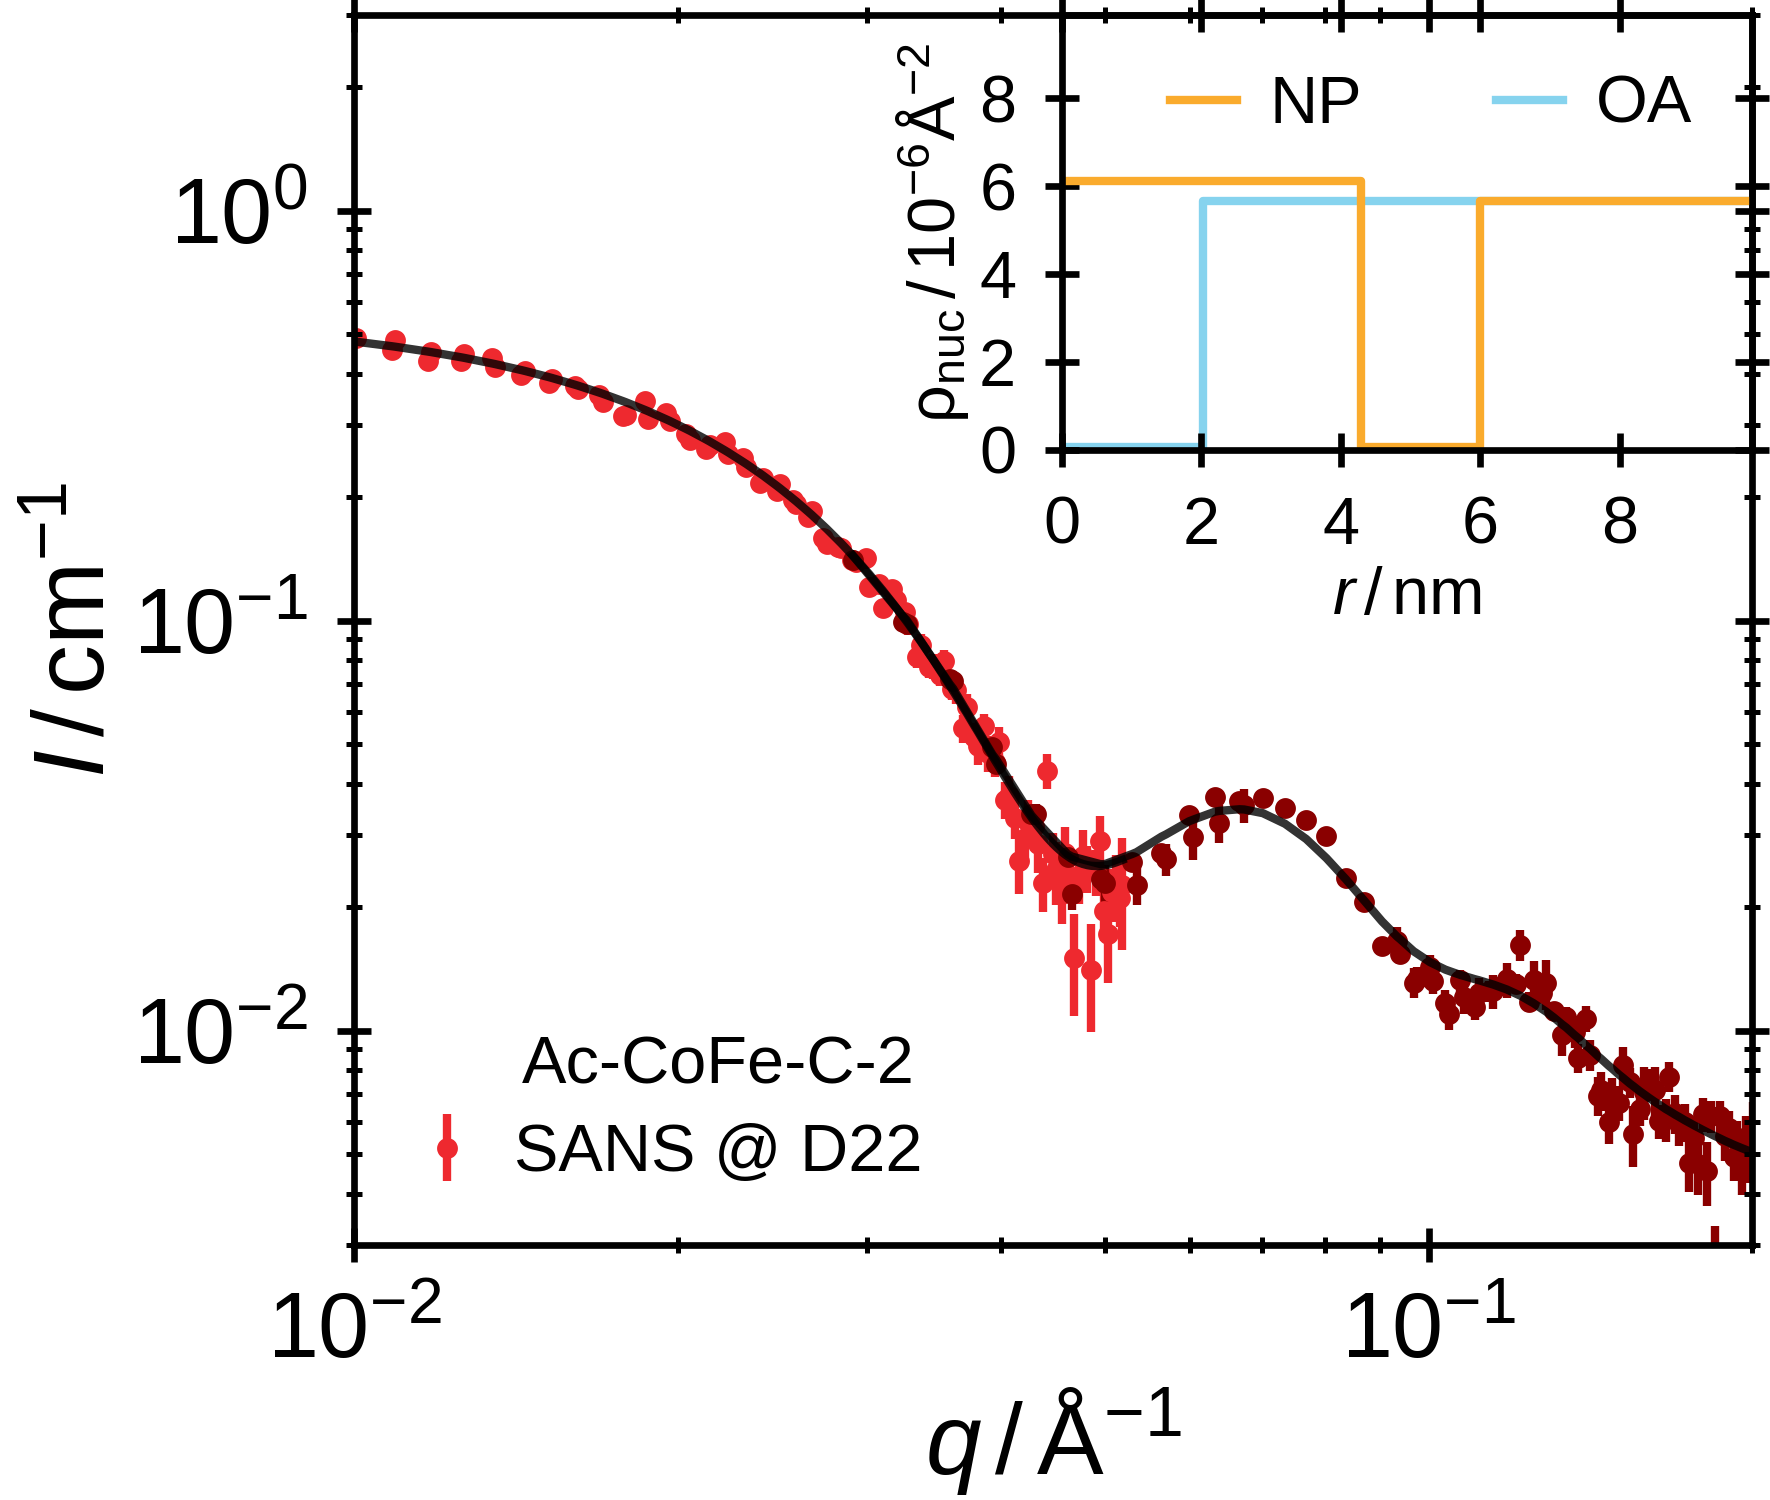
\includegraphics{monolayers_SAS_Ac_CoFe_C_2_SANS}
        \caption{\label{fig:monolayers:nanoparticle:sans:superballOAFit}Ac-CoFe-C (upper) and Ac-CoFe-C-2 (lower) SANS (left) and SANSPOL (right) data described by the sum of a superball form factor and a spherical form factor. The inset shows the SLD profiles of the superball nanoparticles (orange line) and the spherical oleic acid micelles (black).}
      \end{figure}

      \begin{table}[ht]
        \centering
        \caption{\label{tab:monolayers:nanoparticle:sans:superballOAFit}Parameters for the form factors of the sphere, cube and superball shown in \reffig{fig:monolayers:nanoparticle:sas:AcAcCoFeC}.
        The size of the sphere and superball are given in terms of the radius $R$, the size of the cube is given in terms of the edge length $a$.
        The respective log-normal size distribution $\sigma_R$ and $\sigma_a$. $n$ is the particle density in dispersion, $p$ the superball exponent and $\rho_\mathrm{core}$, $\rho_\mathrm{solvent}$ the scattering length densities of the particle and the solvent respectively. The mass concentration $c_m$ of the nanoparticles and oleic acid are determined from the particle number densities and the particle sizes.}
        \begin{tabular}{ c | l | l | l }
          \textbf{SANS}  & \textbf{Ac-CoFe-C} & \textbf{Ac-CoFe-C-2} & \textbf{Ol-CoFe-C}\\
          \hline
          \rule{0pt}{2ex} $d / \unit{nm}$                             & $1.41(3)$      & $1.68(4)$  & $()$ \\
          \rule{0pt}{2ex} $d_\mathrm{OA} / \unit{nm}$                 & $2.34(3)$      & $2.04(8)$  & $()$ \\
          \rule{0pt}{2ex} $n_\mathrm{NP} \, / 10^{-8} \angstrom^{-3}$ & $0.041(2)$     & $0.021(1)$ & $()$ \\
          \rule{0pt}{2ex} $n_\mathrm{OA} \, / 10^{-8} \angstrom^{-3}$ & $0.43(3)$      & $0.41(8)$  & $()$ \\
          \hline
          \rule{0pt}{2ex} $\rho_\mathrm{core}    \, / \unit{10^{-6} \angstrom^{-2}}$   & $6.198$    & $6.132$ & $7.082$\\
          \rule{0pt}{2ex} $\rho_\mathrm{shell}   \, / \unit{10^{-6} \angstrom^{-2}}$   &            &         & $5.938$\\
          \hline
          \rule{0pt}{2ex} $\rho_\mathrm{OA}      \, / \unit{10^{-6} \angstrom^{-2}}$   & \multicolumn{3}{c}{0.078}\\
          \rule{0pt}{2ex} $\rho_\mathrm{solvent} \, / \unit{10^{-6} \angstrom^{-2}}$   & \multicolumn{3}{c}{5.664}\\
          \hline
          \rule{0pt}{2ex} $I_\mathrm{bg} \, / \unit{cm^{-1}}$         & $0.0061(2)$     & $0.0045(3)$        & $0()$\\
          \hline
          \rule{0pt}{2ex} $c_{m, \, \mathrm{NP}} \, / \unit{mg\, mL^{-1}}$ & $1.5(1)$  & $0.58(4)$       & $()$\\
          \rule{0pt}{2ex} $c_{V, \, \mathrm{OA}} \, / \unit{10^{-3}}$      & $0.23(2)$ & $0.15(3)$  & $()$\\
          \hline
          \rule{0pt}{2ex} $\chi^2$                                          & $2.0$      & $2.0$    & $0$\\
          \hline
          \textbf{SANSPOL}\\
          \hline
          \rule{0pt}{2ex} $\rho_\mathrm{mag} \, / \unit{10^{-6} \angstrom^{-2}}$   & $0.97(2)$    & $0$ & $0$\\
          \rule{0pt}{2ex} $M \, / \unit{kA \,m^{-1}}$                       & $334(5)$     & $0$ & $0$\\
          \hline
          \rule{0pt}{2ex} $\chi^2$                                          & $4.4$          & $0$        & $0$\\
        \end{tabular}
      \end{table}
      % 0.041e-2 * (superballVolume(4.69, 2.66) * 5.09 + (superballVolume(4.69+1.41,2.66) - superballVolume(4.69, 2.66))*0.895)
      % 0.041e-2 * (superballVolume(4.69, 2.66) * 5.09 + (0)*0.895)
      % 1.51410663929305

      The best fit shows a good agreement for Ac-CoFe-C with the shell thickness of $1.41 \unit{nm}$ and the average micelles radius of $2.34 \unit{nm}$.

      In \cite{Disch_2010_Thesp}, it is estimated that the head-to-tail distance of oleic acid is $2.1 \unit{nm}$.
      The determined size for the micelles is in a similar order of magnitude, whereas the size for the shell thickness is slightly lower.
      The slightly larger micelle size than the oleic acid chain size, could either  be explained by a small gap in the core of the micelle that is effectively modeled or be due to an insufficient signal-to-noise ratio to properly determine the micelle size.
      The deviation for the nanoparticle shell might be explained due to an intermixing of the oleic acid shell here with the solvent for the nanoparticle surfactant, which is modeled by an effectively reduced shell size, as the oleic acid SLD is fixed to the literature bulk value.

      The determined mass concentration for the nanoparticles is $1.5(1) \unit{mg mL^{-1}}$ and for the oleic acid micelles $0.21(2) \unit{mg mL^{-1}}$.
      The nanoparticle concentration is in agreement with the SAXS value of $1.63(2) \unit{mg mL^{-1}}$.

      For Ac-CoFe-C-2 the same procedure is performed and ...


    \paragraphNewLine{Determination of the core-shell composition for Ol-CoFe-C}
      Due to the core-shell structure of Ol-CoFe-C, the composition of the formula unit is not known from EDX and XRD alone for Ol-CoFe-C.
      As neutrons are highly sensitive to different iron and cobalt content, SANS is additionally used to determine the average formula unit of the nanoparticle core and shell.
      

    \paragraphNewLine{Nanoparticle Magnetization from SANSPOL}
      Given the nuclear model of the scattering length density, the magnetization of the nanoparticles can be determined by fitting the magnetic scattering length density of a magnetic form factor with the same shape and size as used the nuclear form factor using \refeq{eq:methods:sans:sanspolFormula}.
      The obtained fit for $I(+)$ and $I(-)$ is shown in \reffig{fig:monolayers:nanoparticle:sans:superballOAFit} and the values are tabulated in \reftab{tab:monolayers:nanoparticle:sans:superballOAFit}.
      For Ac-CoFe-C a magnetization of $334(5) \unit{kA \, m^{-1}}$ is obtained at $1.2 \unit{T}$ and for Ac-CoFe-C-2 an even higher magnetization of $570 \unit{kA \, m^{-1}}$ is measured.




    % The surfactant shell thickness are in the range of $1 - 2 \unit{nm}$, which is expected for oleic acid chains.
    % As the chains mix with the solvent on the way out, it is expected that the average scattering length density of the shell is not exactly that of bulk oleic acid ($7.8 \cdot 10^{-8} \angstrom^{-2}$), but a mixture with the solvent SLD, which correlates with the model thickness and might explain the reduced value in Ac-CoFe-C.
    % The exact thickness, density and shape of the shell is not of detailed interest for the study of the magnetic properties of the nanocubes and therefore in the scope of this work this rough estimate of the shell is good enough for the discussion.

    % % SANSPOL <-> VSM at 300K
    % The magnetic scattering length density is determined from the SANSPOL data, which is used to determine the magnetization of the nanoparticle using \refeq{eq:looselyPackedNP:nanoparticles:SLDtoMagnetization} to $92(3) \unit{kAm^{-1}}$ for Ol-CoFe-C and $145(2) \unit{kAm^{-1}}$ for Ac-CoFe-C.

    % The fitted model is shown in \reffig{fig:monolayers:nanoparticle:sas:AcAcCoFeC} and the important parameter of interest are given in \reftab{tab:monolayers:nanoparticle:sas} for the following discussion, whereas the full set of model parameters is listed in \refapp{ch:appendix:modelparameters:monolayers:sas_olac_cofe_c}.
    % \begin{table}[ht]
    %   \centering
    %   \caption{\label{tab:monolayers:nanoparticle:sas}Relevant parameters of the superball fit of the small-angle scattering data of the presented nanocubes, the complete set used to describe the models are found in \refapp{ch:appendix:modelparameters:monolayers:sas_olac_cofe_c}.}
    %   \begin{tabular}{ c | l | l }
    %       & Ol-CoFe-C & Ac-CoFe-C \\
    %     \hline
    %     $R$
    %       & $5.62(2) \unit{nm}$
    %       & $4.69(1) \unit{nm}$\\
    %     $\sigma_R$
    %       & $9.27(8) \,\%$
    %       & $11.9(1) \,\%$\\
    %     $D$
    %       & $1.63(1) \unit{nm}$
    %       & $1.16(4) \unit{nm}$\\
    %     $p$
    %       & $1.54(3) \unit{nm}$
    %       & $2.66(9) \unit{nm}$\\
    %     $\rho_\mathrm{mag}^\mathrm{sans}$
    %       & $0.268(8) \cdot 10^{-6} \angstrom^{-2}$
    %       & $0.423(7) \cdot 10^{-6} \angstrom^{-2}$\\
    %     \hline
    %     $V_p$
    %       & $1030(10) \unit{nm^3}$
    %       & $726(5) \unit{nm}$\\
    %     $M^\mathrm{sans}$
    %       & $92(3) \unit{kAm^{-1}}$
    %       & $145(2) \unit{kAm^{-1}}$\\
    %     \hline
    %   \end{tabular}
    % \end{table}
    % The superball model result confirms the qualitative observation that the Ol-CoFe-C nanoparticles have a smaller size distribution than the Ac-CoFe-C cubes.
    % Where the specimen size used to determine size and size distributions in TEM leave the option for a biased result due to possibly missed counting fractions of the dispersion by only measuring a small selected amount of nanoparticles, the large number of particles scanned in the small-angle scattering experiments reveals without bias the average particle size and variation.
    % Furthermore, the model gives that on average Ol-CoFe-C has a higher degree of roundness on the corners, visible from the smaller $p$ parameter in comparison to Ac-CoFe-C.
    % To see this in imaging experiments, high resolution transmission electron microscopy (HR-TEM) experiments are necessary.
    % A study comparing the effectiveness of the superball model in comparison to HR-TEM can be found in \refapp{app:structureCoFe2O4Nanocubes} for three particle batches synthesized similar to Ac-CoFe-C (with a lower heating rate and varied cobalt content, but otherwise same synthesis parameters).
\end{document}